%% 
%% Copyright 2007-2020 Elsevier Ltd
%% 
%% This file is part of the 'Elsarticle Bundle'.
%% ---------------------------------------------
%% 
%% It may be distributed under the conditions of the LaTeX Project Public
%% License, either version 1.2 of this license or (at your option) any
%% later version.  The latest version of this license is in
%%    http://www.latex-project.org/lppl.txt
%% and version 1.2 or later is part of all distributions of LaTeX
%% version 1999/12/01 or later.
%% 
%% The list of all files belonging to the 'Elsarticle Bundle' is
%% given in the file `manifest.txt'.
%% 
%% Template article for Elsevier's document class `elsarticle'
%% with harvard style bibliographic references

%\documentclass[preprint,12pt,authoryear]{elsarticle}
\documentclass[preprint,9pt,authoryear]{elsarticle}

%% Use the option review to obtain double line spacing
%%\documentclass[authoryear,preprint,review,12pt]{elsarticle}

%% Use the options 1p,twocolumn; 3p; 3p,twocolumn; 5p; or 5p,twocolumn
%% for a journal layout:
%% \documentclass[final,1p,times,authoryear]{elsarticle}
%%\documentclass[final,1p,times,twocolumn,authoryear]{elsarticle}
%% \documentclass[final,3p,times,authoryear]{elsarticle}
%% \documentclass[final,3p,times,twocolumn,authoryear]{elsarticle}
%% \documentclass[final,5p,times,authoryear]{elsarticle}
%%\documentclass[final,5p,times,twocolumn,authoryear]{elsarticle}

%% For including figures, graphicx.sty has been loaded in
%% elsarticle.cls. If you prefer to use the old commands
%% please give \usepackage{epsfig}

%% The amssymb package provides various useful mathematical symbols
\usepackage{amssymb}
%% The amsthm package provides extended theorem environments
%% \usepackage{amsthm}

%% The lineno packages adds line numbers. Start line numbering with
%% \begin{linenumbers}, end it with \end{linenumbers}. Or switch it on
%% for the whole article with \linenumbers.
%% \usepackage{lineno}
\usepackage{amsmath}
\usepackage{pgfplotstable,filecontents}
\usepackage{hyperref}
\usepackage{amsmath}
\usepackage{placeins}  % for \FloatBarrier
\usepackage{svg}
\usepackage{caption}
\usepackage{subcaption}
%\usepackage{cancel}
\usepackage{flafter}  % no figures before reference
%\usepackage{layouts}
\usepackage{bm}  % bold text

\journal{International Journal of Naval Architecture and Ocean Engineering}

\begin{document}

\begin{frontmatter}

    %% Title, authors and addresses

    %% use the tnoteref command within \title for footnotes;
    %% use the tnotetext command for theassociated footnote;
    %% use the fnref command within \author or \affiliation for footnotes;
    %% use the fntext command for theassociated footnote;
    %% use the corref command within \author for corresponding author footnotes;
    %% use the cortext command for theassociated footnote;
    %% use the ead command for the email address,
    %% and the form \ead[url] for the home page:
    %% \title{Title\tnoteref{label1}}
    %% \tnotetext[label1]{}
    %% \author{Name\corref{cor1}\fnref{label2}}
    %% \ead{email address}
    %% \ead[url]{home page}
    %% \fntext[label2]{}
    %% \cortext[cor1]{}
    %% \affiliation{organization={},
    %%            addressline={}, 
    %%            city={},
    %%            postcode={}, 
    %%            state={},
    %%            country={}}
    %% \fntext[label3]{}

    %\title{System identification of a physics-informed ship model for better predictions in wind conditions}
    %\title{Virtual Captive Tests for Identifying System-Based Manoeuvring Models}
    \title{Virtual captive tests for standard ship manoeuvres}
    

    %% use optional labels to link authors explicitly to addresses:
    %% \author[label1,label2]{}
    %% \affiliation[label1]{organization={},
    %%             addressline={},
    %%             city={},
    %%             postcode={},
    %%             state={},
    %%             country={}}
    %%
    %% \affiliation[label2]{organization={},
    %%             addressline={},
    %%             city={},
    %%             postcode={},
    %%             state={},
    %%             country={}}

    \author[1,2]{Martin Alexandersson\corref{cor1}%
        %\fnref{fn1,fn3}
    }
    \ead{maralex@chalmers.se}
    \author[1]{Wengang Mao}
    \author[1]{Jonas W. Ringsberg}
    \author[2]{Martin Kjellberg}


    \affiliation[1]{organization={Dept. of Mechanics and Maritime Sciences, Division of Marine Technology, Chalmers University of Technology},%Department and Organization
        addressline={Hörsalsvägen 7A},
        city={Gothenburg},
        postcode={41296},
        country={Sweden}}


    \affiliation[2]{organization={Research Institutes of Sweden (RISE), SSPA Maritime Center},%Department and Organization
        addressline={Chalmers tvärgata 10},
        city={Gothenburg},
        postcode={41296},
        country={Sweden}}

    \cortext[cor1]{Corresponding author}

    \begin{abstract}
        Ships with wind-assisted propulsion systems (WAPS) should be equipped with large rudders to compensate for WAPS-induced drifting forces. The WAPS also significantly affects the effectiveness of mathematical models used to describe the ship's maneuvering characteristics. In this study, the Maneuvering Modeling Group (MMG) is chosen and various approaches are proposed to identify different parameters within the MMG model. First, the ship's hydrodynamic coefficients, such as mass, added mass, and center of gravity, are estimated from either model tests or hydrodynamic analysis. The hydrodynamic forces and drifting forces are proposed to be analyzed by virtual captive tests (VCT). The key part of identifying MMG models for ships with WAPS is to obtain accurate rudder forces. Various explicit semi-empirical formulas are proposed to approximate the rudder forces when experimental data on the rudder forces is not available. Based on the experimental tests with rudder forces measured, the quadratic semi-empirical models are found to perfectly describe such forces. Finally, the other parameters in the MMG model are estimated by the inverse dynamics based on the series of maneuvering tests. In this study, two ships designed with WAPS, i.e., wPCC and Optiwise, are used to validate the proposed method based on their experimental model tests. For the wPCC ship with double rudders, large discrepancies are observed between the close loop maneuvering prediction by the identified model and tests, due to the incapability of VCTs to model rudder forces, and asymmetric patterns of flows on the two rudders. When the measurement of rudder forces is available for the Optiwise ship, the MMG model identified by the proposed method can perfectly predict the ship’s maneuvering motions compared to the tests.
% Move 1 - Background/introduction/situation

% Move 2 - Present research/purpose

% Move 3 - Methods/materials/subjects/procedures

% Move 4 - Results/findings

% Move 5 - Discussion/conclusion/significance

    \end{abstract}

    %%Graphical abstract
    %\begin{graphicalabstract}
    %    %\includegraphics{grabs}
    %\end{graphicalabstract}
    %
    %%%Research highlights
    %\begin{highlights}
    %    \item Research highlight 1
    %    \item Research highlight 2
    %\end{highlights}

    \begin{keyword}
    Inverse dynamics \sep Physics-informed maneuvering model \sep System identification \sep Wind-assisted propulsion 
        %% keywords here, in the form: keyword \sep keyword

        %% PACS codes here, in the form: \PACS code \sep code

        %% MSC codes here, in the form: \MSC code \sep code
        %% or \MSC[2008] code \sep code (2000 is the default)

    \end{keyword}

\end{frontmatter}
%% \linenumbers
%textwidth in inches: \printinunitsof{in}\prntlen{\textwidth} \newline
%textheight in inches: \printinunitsof{in}\prntlen{\textheight}
%% main text
%\newpage
\section*{Nomenclature}
\label{sec:introduction}
\begin{table}[h]
    \centering
    %\footnotesize
    \scriptsize
    %\caption{Semi-empirical rudder parameters (SI units) in model scale.}
    \label{tab:other_parameters}
    \pgfplotstabletypeset[col sep=comma, column type=r,
    columns/LaTeX/.style={column type=r,string type,column name=~},
    columns/LaTeX1/.style={column type=r,string type, column name=~},
    columns/LaTeX2/.style={column type=r,string type, column name=~},
    %columns/LaTeX3/.style={column type=l,string type, column name=~},
    columns/Description/.style={column type=p{3.3cm},string type,column name=~},
    columns/Description1/.style={column type=p{3.3cm},string type, column name=~},
    columns/Description2/.style={column type=p{3.3cm},string type, column name=~},
    %columns/Description3/.style={column type=l,string type, column name=~},
    %every head row/.style={before row=\hline,after row=\hline},
    %every last row/.style={after row=\hline}
    ]{tables/mathematical_model_kinetics.nomenclature.csv}
\end{table}
\FloatBarrier

\section*{Abbreviations}
\label{sec:introduction}
\begin{table}[h]
    \centering
    %\footnotesize
    \scriptsize
    %\caption{Semi-empirical rudder parameters (SI units) in model scale.}
    \label{tab:abbreviations}
    \begin{tabular}{l l}

    CFD & Computational fluid dynamics \\
    CMT & Captive model tests \\
    FRMT & Free running model tests \\
    ID & Inverse dynamics \\
    MMG & Manoeuvring modeling group \\
    OLS & Ordinary least-square \\
    RHI & Rudder hull interaction \\
    VCT & Virtual captive tests \\
    wPCC & Wind powered car carrier \\
    \end{tabular}
        
\end{table}
\FloatBarrier


\section{Introduction}
\label{sec:introduction}
\section{Model}
\begin{figure}[h]
    \centering
    \includesvg{figures/reference_frames.svg}
    \caption{Relations between the earth fixed and ship fixed reference frames, showing the velocities and forced in the ship fixed frame.}
    \label{fig:reference_frames}
\end{figure}
\noindent The kinematics of a ship is expressed in the middle of the ship in a ship fixed coordinate system, rotated around the Earth-fixed coordinate system $x_0$, $y_0$ by the heading angle $\Psi$ as shown in \autoref{fig:reference_frames}. 
\begin{figure}[h!]
    \centering
    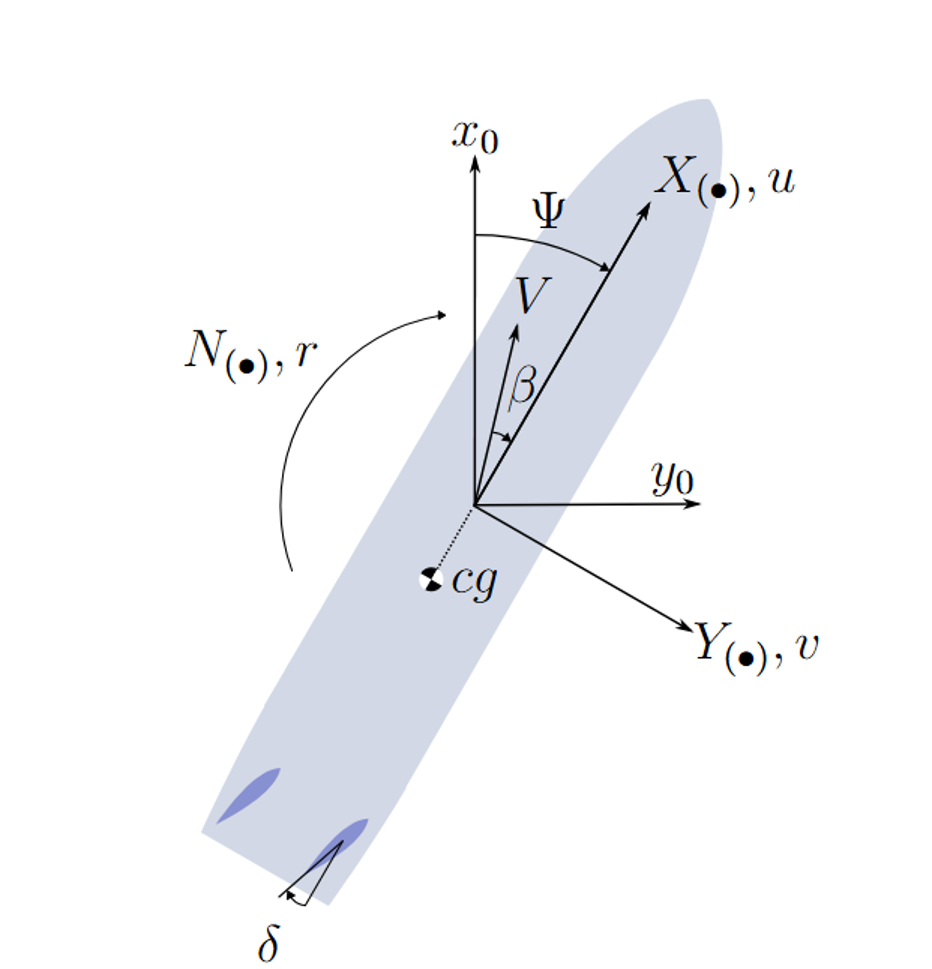
\includegraphics[width=6cm, height=6cm]{figures/reference_frames.png}
    \caption{Ship velocities and forces in the Earth-fixed and ship-fixed coordinate systems.}
    \label{fig:reference_frames}
\end{figure}
Forces and motions are expressed in three degrees of freedom, that is, surge $X$, sway $Y$, and yaw $N$. During a ship's maneuvering, since the forces do not depend on the position ($x_0,y_0$) or heading $\Psi$, the kinematics and motion equations of the ship can be expressed as a function of the velocity vector $\pmb{\bm{\upsilon}}$ as
% \begin{equation}
%     \label{eq:upsilon}
%     %\upsilon = \left[\begin{matrix}u\\v\\r\end{matrix}\right]
%     \pmb{\bm{\upsilon}} = \left[\begin{matrix}u\\v\\r\end{matrix}\right]
% \end{equation}
% The equation of motion can thus be expressed as \autoref{eq:eom}
\begin{equation}
    \label{eq:eom}
    \mathbf{F} = \mathbf{M}  \pmb{\bm{\dot{\upsilon}}}, \hspace{1cm}
    \pmb{\bm{\upsilon}} = \left[\begin{matrix}u\\v\\r\end{matrix}\right]
\end{equation}
where $\pmb{\bm{\dot{\upsilon}}}$ is the acceleration vector, $\mathbf{M}$ is the system inertia matrix and $\mathbf{F}$ is the total force vector.
% The velocity transition can thus be expressed as
% \begin{equation}
%     \label{eq:acc}
%     \pmb{\bm{\dot{\upsilon}}} = \mathbf{M}^{-1}\mathbf{F}
% \end{equation}
The total forces can be divided into the Coriolis–centripetal matrix $\mathbf{C}$ and the damping force vector $\mathbf{D}$ \citep{fossenHandbookMarineCraft2011}, while the control forces from the rudder and propeller are included in the $\mathbf{D}$ matrix as follows,
\begin{equation}
    \label{eq:C_expanded}
    \mathbf{C} = \left[\begin{matrix}0 & - m r & Y_{\dot{r}} r + Y_{\dot{v}} v - m r x_{G}\\m r & 0 & - X_{\dot{u}} u\\- Y_{\dot{r}} r - Y_{\dot{v}} v + m r x_{G} & X_{\dot{u}} u & 0\end{matrix}\right], \hspace{0.3cm}
    \mathbf{D} = \left[\begin{matrix}X_{D}\\Y_{D}\\N_{D}\end{matrix}\right]
\end{equation}
% \begin{equation}
%     \label{eq:D}
%     \mathbf{D} = \left[\begin{matrix}X_{D}\\Y_{D}\\N_{D}\end{matrix}\right]
% \end{equation}
where the added masses  $X_{\dot{u}},Y_{\dot{v}},Y_{\dot{r}},N_{\dot{v}},N_{\dot{r}} < 0$, then the total force vector $\mathbf{F}$ can now be expressed as:
\begin{equation}
    \label{eq:F_expanded}
    %F = \mathbf{D} + \mathbf{\tau_{wave}} + \mathbf{\tau_{wind}} + \mathbf{\tau} + \left[\begin{matrix}m r v - r \left(Y_{\dot{r}} r + Y_{\dot{v}} v - m r x_{G}\right)\\X_{\dot{u}} r u - m r u\\- X_{\dot{u}} u v - u \left(- Y_{\dot{r}} r - Y_{\dot{v}} v + m r x_{G}\right)\end{matrix}\right]
\mathbf{F} = - \mathbf{C} \upsilon + \mathbf{D} =
\left[\begin{matrix}
X \\
Y \\
N \\
\end{matrix}\right]
=
\left[\begin{matrix}X_{D} - Y_{\dot{r}} r^{2} + m r^{2} x_{G} + r v \left(- Y_{\dot{v}} + m\right)\\Y_{D} + r u \left(X_{\dot{u}} - m\right)\\N_{D} + r u \left(Y_{\dot{r}} - m x_{G}\right) + \underbrace{u v \left(- X_{\dot{u}} + Y_{\dot{v}}\right)}_{\text{Munk moment}} \end{matrix}\right]
\end{equation}
where $u v \left(- X_{\dot{u}} + Y_{\dot{v}}\right)$ in the yawing moment $N$ is the so called Munk moment \citep{fossenHandbookMarineCraft2011}; $r u \left(X_{\dot{u}} - m\right)$ in the sway force $Y$ has the apparent centrifugal force from added mass and rigid body mass with $X_{\dot{u}}<0$, so that both added mass and rigid body mass create the centrifugal force acting outward in the turn. Both the added mass and rigid body mass will thus act to starboard on a port turn.
% \begin{equation}
%     \label{eq:upsilon1d}
% \mathbf{F} = - \mathbf{C} \upsilon + \mathbf{D}
% \end{equation}

For the calculation of acceleration $\pmb{\bm{\dot{\upsilon}}}$ in \autoref{fig:reference_frames}, the mass matrix $\mathbf{M}$ and its inverse can be calculated according to \citet{fossenHandbookMarineCraft2011} as shown in, 
\begin{equation}
    \label{eq:M_expanded}
    \mathbf{M} = \left[\begin{matrix}- X_{\dot{u}} + m & 0 & 0\\0 & - Y_{\dot{v}} + m & - Y_{\dot{r}} + m x_{G}\\0 & - N_{\dot{v}} + m x_{G} & I_{z} - N_{\dot{r}}\end{matrix}\right],
   % \frac{1}{\mathbf{M}} = \left[\begin{matrix}\frac{1}{- X_{\dot{u}} + m} & 0 & 0\\0 & \frac{- I_{z} + N_{\dot{r}}}{S} & \frac{- Y_{\dot{r}} + m x_{G}}{S}\\0 & \frac{- N_{\dot{v}} + m x_{G}}{S} & \frac{Y_{\dot{v}} - m}{S}\end{matrix}\right]
\end{equation}
% \begin{equation}
%     \label{eq:M_inv}
%     \frac{1}{\mathbf{M}} = \left[\begin{matrix}\frac{1}{- X_{\dot{u}} + m} & 0 & 0\\0 & \frac{- I_{z} + N_{\dot{r}}}{S} & \frac{- Y_{\dot{r}} + m x_{G}}{S}\\0 & \frac{- N_{\dot{v}} + m x_{G}}{S} & \frac{Y_{\dot{v}} - m}{S}\end{matrix}\right]
% \end{equation}
% the helper variable $S = I_{z} Y_{\dot{v}} - I_{z} m - N_{\dot{r}} Y_{\dot{v}} + N_{\dot{r}} m + N_{\dot{v}} Y_{\dot{r}} - N_{\dot{v}} m x_{G} - Y_{\dot{r}} m x_{G} + m^{2} x_{G}^{2}$.
% \begin{equation}
%     \label{eq:S}
%     S = I_{z} Y_{\dot{v}} - I_{z} m - N_{\dot{r}} Y_{\dot{v}} + N_{\dot{r}} m + N_{\dot{v}} Y_{\dot{r}} - N_{\dot{v}} m x_{G} - Y_{\dot{r}} m x_{G} + m^{2} x_{G}^{2}
% \end{equation}
%\vspace{0.5cm}



The damping forces and moments are expressed in a modular way, as shown in \autoref{eq:X_D}--\autoref{eq:N_D} and \autoref{fig:force_model},
% Components:
\begin{equation}
    \label{eq:X_D}
    X_{D} = X_{H} + X_{P} + X_{R}
\end{equation}
%
\begin{equation}
    \label{eq:Y_D}
    Y_{D} = Y_{H} + Y_{P} + Y_{R} + Y_{RHI}
\end{equation}
%
\begin{equation}
    \label{eq:N_D}
    N_{D} = N_{H} + N_{P} + N_{R} + N_{RHI}
\end{equation}
%
\begin{figure}[h]
    \centering
    \includesvg[width=4cm]{figures/force_model.svg}
    \caption{Modular force components.}
    \label{fig:force_model}
\end{figure}
where subscripts $H$, $P$, $R$, and $RHI$ represent contributions from the hull, propellers, rudders, and rudder hull interaction, respectively. The rudder hull interaction having its own element is a difference from the MMG model.
\subsection{Hull}
\noindent Based on the above-mentioned prime system, the hydrodynamic forces acting on a ship's hull as in \autoref{eq:XYN_H} can be described viz,
\begin{equation}
    \label{eq:XYN_H}
    \left.\begin{aligned}
    X_H & = 1/2\rho L^{2} U^{2} X_H^{'}  \\
    Y_H & = 1/2\rho L^{2} U^{2} Y_H^{'}  \\
    N_H & = 1/2\rho L^{3} U^{2} X_H^{'}
    \end{aligned}\right\}
\end{equation}
where the non-dimensional surge force $X_H^{'}$, lateral force $Y_H^{'}$ and yaw moment $N_H^{'}$ are normally modeled by the following general polynomials in terms of non-dimensional velocities $u^{'}, v^{'}$ and yaw rate $r'$ based on the MMG model, \citep{yasukawaIntroductionMMGStandard2015},
\begin{equation}
    \label{eq:XYN_H_prime}
    \left.\begin{aligned}
    {X_H'} = {X_{0}'} + {X_{rr}'} {r'}^{2} + {X_{u}'} {u'} + {X_{vr}'} {r'} {v'} + {X_{vv}'} {v'}^{2} \\
    {Y_H'} = {Y_{0}'} + {Y_{rrr}'} {r'}^{3} + {Y_{r}'} {r'} + {Y_{vrr}'} {r'}^{2} {v'} + {Y_{vvr}'} {r'} {v'}^{2} + {Y_{vvv}'} {v'}^{3} + {Y_{v}'} {v'} \\
    {N_H'} = {N_{0}'} + {N_{rrr}'} {r'}^{3} + {N_{r}'} {r'} + {N_{vrr}'} {r'}^{2} {v'} + {N_{vvr}'} {r'} {v'}^{2} + {N_{vvv}'} {v'}^{3} + {N_{v}'} {v'}
    \end{aligned}\right\}
\end{equation}
where the coefficients $X_0^{'}, X_{rr}^{'}, X_u^{'}, X_{vr}^{'}, X_{vv}^{'}, Y_{0}^{'}, Y_{rrr}^{'}, Y_{r}^{'}, Y_{vrr}^{'}, Y_{vvr}^{'}, Y_{vvv}^{'}, Y_{v}^{'}, N_{0}^{'}$, $N_{rrr}^{'}$, $N_{r}^{'}$, $N_{vrr}^{'}$, $N_{vvr}^{'}$, $N_{vvv}^{'}$, $N_{v}^{'}$ are referred to as the hydrodynamic derivatives on ship manoeuvring. They represent the impact of different velocity components to the three hydrodynamic forces on the ship's hull. An important task for system identification of ship manoeuvring in this study is to find those derivatives. Furthermore, in this study, the perturbed surge velocity is proposed to allow for the extra resistance term ${X_u}'$, so that the resistance curve does not need to have a quadratic shape as in the MMG model.  
%
% \begin{equation}
%     \label{eq:Y_H}
%     {Y_H'} = {Y_{0}'} + {Y_{rrr}'} {r'}^{3} + {Y_{r}'} {r'} + {Y_{vrr}'} {r'}^{2} {v'} + {Y_{vvr}'} {r'} {v'}^{2} + {Y_{vvv}'} {v'}^{3} + {Y_{v}'} {v'}
% \end{equation}
% %
% \begin{equation}
%     \label{eq:N_H}
%     {N_H'} = {N_{0}'} + {N_{rrr}'} {r'}^{3} + {N_{r}'} {r'} + {N_{vrr}'} {r'}^{2} {v'} + {N_{vvr}'} {r'} {v'}^{2} + {N_{vvv}'} {v'}^{3} + {N_{v}'} {v'}
% \end{equation}
\subsection{Rudder}
\noindent In the MMG model introduced in \citet{yasukawaIntroductionMMGStandard2015}, if the rudder tangential force is neglected, the effective rudder forces $X_R, Y_R$ and $N_R$ can be described as:
\begin{equation}
   \label{eq:rudder}
  \left.\begin{aligned}
  X_R & = - (1-t_R) F_N \sin \delta\\
  Y_R & = - (1+ \alpha_H) F_N \cos \delta\\
  N_R & = - (x_R + \alpha_H x_H) F_N \cos \delta
\end{aligned}\right\}
\end{equation}
where $F_N$ denotes the hydrodynamic forces applied on the normal direction of the rudder, $\delta$ denotes the rudder angle, and $t_R$, $\alpha_H$, $x_R, x_H$ denote the coefficients describing hydrodynamic interaction between rudder and hull, while $x_R, x_H$ represent longitudinal locations of the additional lateral forces applied on rudder and ship hull, respectively. The semi-empirical models for these coefficients are described in detail in \citet{yasukawaIntroductionMMGStandard2015} and \citet{alexanderssonSystemIdentificationPhysicsinformed2024b}. The key component in estimating effective rudder forces in Eq.(\ref{eq:rudder}) is to obtain the normal force applied on the rudder expressed by:
\begin{equation}
    \label{eq:rudder_normal}
    F_N & = 1/2 \rho A_R U_R^{2} f_{\alpha} \sin \alpha_R
\end{equation}
where $A_R, f_\alpha$ denote the rudder area and the rudder lift gradient coefficient, respectively, and $\alpha_R$ is the angle of effective flow to the rudder, which has significant impact on the rudder force in Eq.(\ref{eq:rudder_normal}) due the asymmetric properties of flows caused by ship drifting.
In this study, a new quadratic rudder model is proposed with two enhancements to the original MMG rudder model as in \citet{yasukawaIntroductionMMGStandard2015}  in order to get a better fit to the VCT data. The first enhancement is to add the angle of initial inflow to rudder  $\gamma_0$ for the calculation of the angle of effective inflow acting to rudder $\alpha_R$:  
\begin{equation}
    \label{eq:alpha_R2}
    %\alpha_{R} = \delta + \gamma_{0} + \operatorname{atan}{\left(\frac{v_{R}}{u_{R}} \right)}
    \alpha_{R} = \delta + \underbrace{\gamma_{0}}_{~} + \operatorname{atan}{\left(\frac{v_{R}}{u_{R}} \right)}
\end{equation}
which allows the rudder model to produce a side force in the straight ahead condition, due to unsymmetrical flow from the propeller.

The other enhancement is to allow for a quadratic relationship between the flow straightening coefficient $\gamma_R$ and the effective inflow angle $\beta_R$ by introducing two new coefficients $\gamma_{R2neg}$, and $\gamma_{R2pos}$ as:  
\begin{equation}
    \label{eq:gamma_R2}
    \gamma_{R} = \begin{cases} \gamma_{R2 neg} \left|{\beta_{R}}\right| + \gamma_{R neg} & \text{for}\: \beta_{R} \leq 0 \\\gamma_{R2 pos} \left|{\beta_{R}}\right| + \gamma_{R pos} & \text{otherwise} \end{cases}
\end{equation}
which can be used to calculate the transverse velocity of flow passing the rudder as in Eq.(\ref{eq:alpha_R2}). 



\section{Methodology}
\subsection{Inertia}
\noindent The mass properties of the ship models, including the added masses, need to be determined in order to conduct simulations or inverse dynamics. The rigid body mass and mass inertia were determined with swing tests in air before the FRMTs were carried out at RISE Maritime Dynamics Laboratory (MDL) in Gothenburg (Sweden). The vertical center of gravity was determined with inclining experiments with the scale models in the MDL basin.

In this study, it is proposed to determine the added mass of the yaw $N_{\dot{r}}$ with the Fourier series method \citep{sakamotoURANSSimulationsStatic2012} applied to a pure yaw test carried out in a fully non-linear potential flow panel method (FNPF) in ShipFlow Motions \citep{kjellbergFullyNonlinearUnsteady2013}.
ShipFlow Motions uses a fully nonlinear boundary element method solver for computing ship motions with better accuracy than traditional potential flow methods while being faster than the available CFD (computational fluid dynamics) methods.
During the pure yaw test the heading $\Psi$ was varied  so that the yaw rate $r$ and yaw acceleration $\dot{r}$ were varied as:
\begin{equation}
    \left.\begin{aligned}
    \Psi = - \Psi_{max} \cos{\left(t w \right)} \\
    r = \Psi_{max} w \sin{\left(t w \right)} \\
    \dot{r} = \Psi_{max} w^{2} \cos{\left(t w \right)}
    \end{aligned}\right\}.
    \label{eq:pure_yaw_psi}
\end{equation}
% \begin{equation}
%     r = \Psi_{max} w \sin{\left(t w \right)}
%     \label{eq:pure_yaw_r}
% \end{equation}
% \begin{equation}
%     \dot{r} = \Psi_{max} w^{2} \cos{\left(t w \right)}
%     \label{eq:pure_yaw_r1d}
% \end{equation}
The pure yaw calculations in Shipflow Motions were conducted without propeller and rudder so that $N_D=N_H$ and the moment equilibrium with the yawing moment from the pressure integration in Shipflow Motions $N_M$ could be expressed as: 
\begin{equation}
    N_{M} = N_{\dot{r}} \dot{r} + N_{rrr} r^{3} + N_{r} r + Y_{\dot{r}} r u
    \label{eq:MOTIONS_N}
\end{equation}
where the yaw added mass $N_{\dot{r}}$ was the coefficient of interest. 
The time series for the yawing moment during the pure yaw test could thus be expressed by inserting \autoref{eq:pure_yaw_psi}  into \autoref{eq:MOTIONS_N} as:
\begin{equation}
    N_{M} = N_{\dot{r}} \Psi_{max} w^{2} \cos{\left(t w \right)} + N_{rrr} \Psi_{max}^{3} w^{3} \sin^{3}{\left(t w \right)} + N_{r} \Psi_{max} w \sin{\left(t w \right)} + Y_{\dot{r}} \Psi_{max} u w \sin{\left(t w \right)}
    \label{eq:MOTIONS_N_expanded}
\end{equation}
which can instead be expressed as a Fourier series with three components as:
\begin{equation}
    N_M = N_0 + \sum_{n=1}^3a_n \cos(n \omega t) + \sum_{n=1}^3b_n \sin(n \omega t) 
    \label{eq:fourier}
\end{equation}
in which $N_{\dot{r}}$ can be calculated from the first cosine coefficient viz.:
\begin{equation}
    N_{\dot{r}} = \frac{a_1}{\Psi_{max} w^{2}}
    \label{eq:N_r1d}
\end{equation}
An example of the fitted Fourier series is shown in \autoref{fig:fourier}. The sway added mass $Y_{\dot{v}}$ was determined in a similar way, but instead by conducting a pure sway test. The coupled added masses $N_{\dot{v}}$, and $Y_{\dot{r}}$ were determined with strip theory calculations using the Franks close fit method. 
\begin{figure}[h!]
    \centering   \includesvg[width = 3in]{figures/methodology_pure_yaw_no_FFT.reconstruction.svg}
    \caption{Fourier series fit to the pure yaw Motions results to determine the yaw added mass for wPCC.}
    \label{fig:fourier}
\end{figure}
%\subsection{VCT matrix for wPCC}
%\begin{table}[h]
    \centering
    \small
    \caption{VCT variations for wPCC.}
    \label{tab:inflow_to_rudder_force}
    \pgfplotstabletypeset[col sep=comma, column type=c, style=string type,
        columns/Test type/.style={column type=l,string type},
        columns/V/.style={column type=c,string type, column name=$V$ [m/s]},
        columns/beta_deg/.style={column type=c,string type, column name=$\beta$ [deg]},
        columns/r/.style={column type=c,string type, column name=$r$ [rad/s]},
        columns/delta_deg/.style={column type=c,string type, column name=$\delta$ [deg]},
        columns/rev/.style={column type=c,string type, column name=rev [1/s]},
        %columns/r/.style={column type=r,fixed,fixed zerofill,precision=2, column name=$r$ [rad/s]},
        %columns/V_R/.style={fixed,fixed zerofill,precision=2, column name=$V_R$ [m/s]},
        %columns/gamma_deg/.style={fixed,fixed zerofill,precision=1, column name=$\gamma$ [deg]},
        %columns/Y_R/.style={fixed,fixed zerofill,precision=1, column name=$Y_R^{VCT}$ [N]},
        %columns/Y_R_MMG/.style={fixed,fixed zerofill,precision=1, column name=$Y_R^{MMG}$ [N]},
        every head row/.style={before row=\hline,after row=\hline},
        every last row/.style={after row=\hline}
    ]{tables/methodology_VCT_wPCC.variations.csv}
\end{table}

\begin{figure}[h]
    \includesvg{figures/methodology_VCT_wPCC.phase_plot.svg}
    \caption{Phase plots of the wPCC zigzag tests together with the coverage of the VCTs and extra state VCTs.}
    \label{fig:VCT_phase_plot_wPCC}
\end{figure}
\subsection{Inverse dynamics analysis}
\subsection{state VCT}
\subsection{Hydrodynamic forces from VCT}
VCT calculations are conducted by solving a set of static flow calculations with CFD. The VCT test matrix is selected to have a good coverage of the states that the ship will have during the manoeuvre. How the combinations of drift angle and yaw rate have been selected can be seen in the figure below, for the wPCC. 
The total forces from the VCT $X_{VCT}$, $Y_{VCT}$, and $N_{VCT}$ are recalculated in the following way, to obtain the damping forces.
\begin{equation}
    \label{eq:X_D}
    X_{D} = X_{VCT} + Y_{\dot{r}} r^{2} + Y_{\dot{v}} r v
\end{equation}
\begin{equation}
    \label{eq:Y_D}
    Y_{D} = - X_{\dot{u}} r u + Y_{VCT}
\end{equation}
\begin{equation}
    \label{eq:N_D}
    N_{D} = N_{VCT} + X_{\dot{u}} u v - Y_{\dot{r}} r u - Y_{\dot{v}} u v
\end{equation}
The mass $m$ has disappeared from \autoref{eq:F_expanded} to arrive at these expressions, because the ship is not moving in ShipFlow, instead the water is.
\begin{table}[h]
    \centering
    \small
    \caption{VCT variations for Optiwise.}
    \label{tab:VCT_optiwise}
    \pgfplotstabletypeset[col sep=comma, column type=c, style=string type,
        columns/Test type/.style={column type=l,string type},
        columns/V/.style={column type=c,string type, column name=$V$ [m/s]},
        columns/beta_deg/.style={column type=c,string type, column name=$\beta$ [deg]},
        columns/r/.style={column type=c,string type, column name=$r$ [rad/s]},
        columns/delta_deg/.style={column type=c,string type, column name=$\delta$ [deg]},
        columns/rev/.style={column type=c,string type, column name=rev [1/s]},
        %columns/r/.style={column type=r,fixed,fixed zerofill,precision=2, column name=$r$ [rad/s]},
        %columns/V_R/.style={fixed,fixed zerofill,precision=2, column name=$V_R$ [m/s]},
        %columns/gamma_deg/.style={fixed,fixed zerofill,precision=1, column name=$\gamma$ [deg]},
        %columns/Y_R/.style={fixed,fixed zerofill,precision=1, column name=$Y_R^{VCT}$ [N]},
        %columns/Y_R_MMG/.style={fixed,fixed zerofill,precision=1, column name=$Y_R^{MMG}$ [N]},
        every head row/.style={before row=\hline,after row=\hline},
        every last row/.style={after row=\hline}
    ]{tables/methodology_VCT_optiwise.variations.csv}
\end{table}
\begin{figure}[h]
    \includesvg{figures/methodology_VCT_optiwise.phase_plot.svg}
    \caption{Phase plots of the Optiwise zigzag tests together with the coverage of the VCTs and extra state VCTs.}
    \label{fig:VCT_phase_plot_optiwise}
\end{figure}
\FloatBarrier
\subsection{wPCC test case}
The wPCC has wind-assisted ship propulsion (WASP) and can alter between a fully sailing mode, and a fully motoring mode, and in between. 
However, this paper only considers the motoring mode. Because of the WASP, the wPCC design differs slightly from conventional motoring cargo ship designs. The wPCC has two very large rudders, two to three times larger than needed for a conventional ship. The ship also has fins at the bilge to generate extra lift while sailing, as shown on the scale model in \autoref{fig:wPCC}. 
%This figure also show two fans, that can be used to simulate wind forces, these were however not used in the manoeuvring tests of this paper. 
\autoref{tab:main_particulars} shows the main particulars of the scale model. 
\begin{figure}[h]
    \centering
    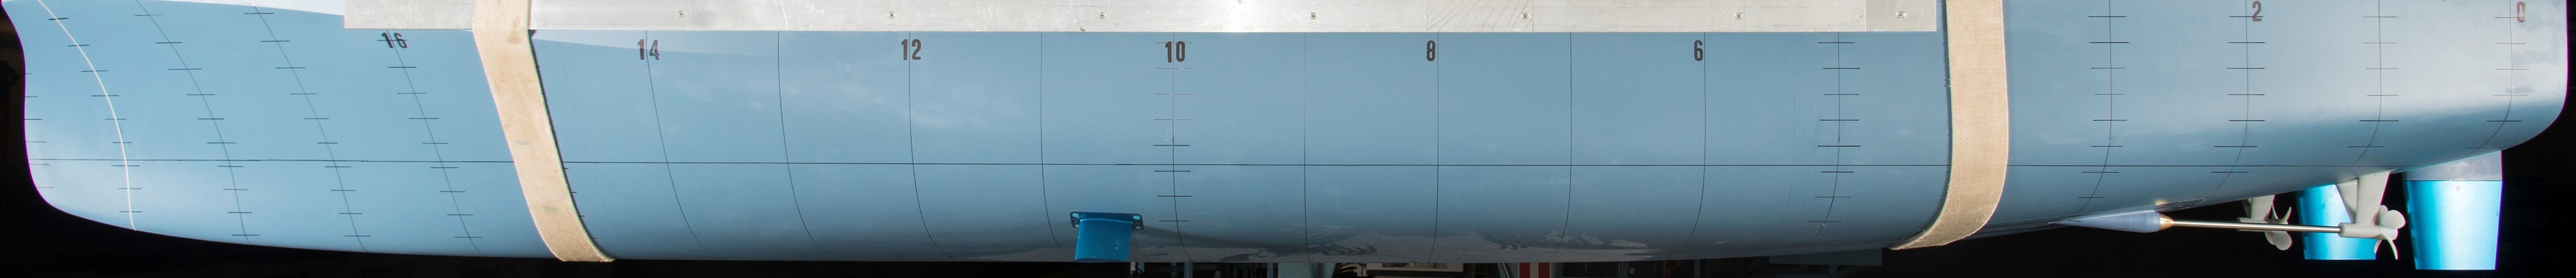
\includegraphics[width=\columnwidth]{figures/5m2.jpg}
    \caption{Scale model of the wPCC used in the model tests. Copyright RISE.}
    \label{fig:wPCC}
\end{figure}
Required input parameters for the semi-empirical rudder model are summarized in \autoref{tab:other_parameters}.
\begin{table}[h]
    \centering
    \caption{Main particulars (SI units) of the wPCC scale model.}
    \label{tab:main_particulars}
    \pgfplotstabletypeset[col sep=comma, column type=r,
        columns/Parameter/.style={column type=l,string type},
        columns/Unit/.style={column type=l,string type,column name=~},
        columns/Description/.style={column type=l,string type},
        columns/Value/.style={column type=r, column name=~},
        every head row/.style={before row=\hline,after row=\hline},
        every last row/.style={after row=\hline}
    ]{tables/result_models.main_particulars.csv}
\end{table}
\subsection{Optiwise test case}
\FloatBarrier


\section{Results}
\label{sec:results}
%\input{result}
\FloatBarrier

%\subsection{VCT wPCC}
%\begin{figure}[h]
     \centering
     \begin{subfigure}[b]{0.49\textwidth}
         \centering
         \includesvg[width=0.99\textwidth]{figures/results_wPCC_VCT.drift_angle_X.svg}
        \caption{Surge.}
        \label{fig:drift_angle_X}
     \end{subfigure}
     \hfill
     \begin{subfigure}[b]{0.49\textwidth}
         \centering
         \includesvg[width=0.99\textwidth]{figures/results_wPCC_VCT.drift_angle_Y.svg}
        \caption{Sway.}
        \label{fig:drift_angle_Y}
     \end{subfigure}
     \vfill
     \begin{subfigure}[b]{\textwidth}
         \centering
         \includesvg{figures/results_wPCC_VCT.drift_angle_N.svg}
        \caption{Yawing moment.}
        \label{fig:drift_angle_N}
     \end{subfigure}
    \caption{Overshoot angles from the wPCC experiments and simulations.}
    \label{fig:overshoots_wPCC}
\end{figure}


The flow from the port dagger board hits the starboard rudder for 15 degrees drift angle as shown in \autoref{fig:streamlines15}.
\begin{figure}[h]
    \centering
    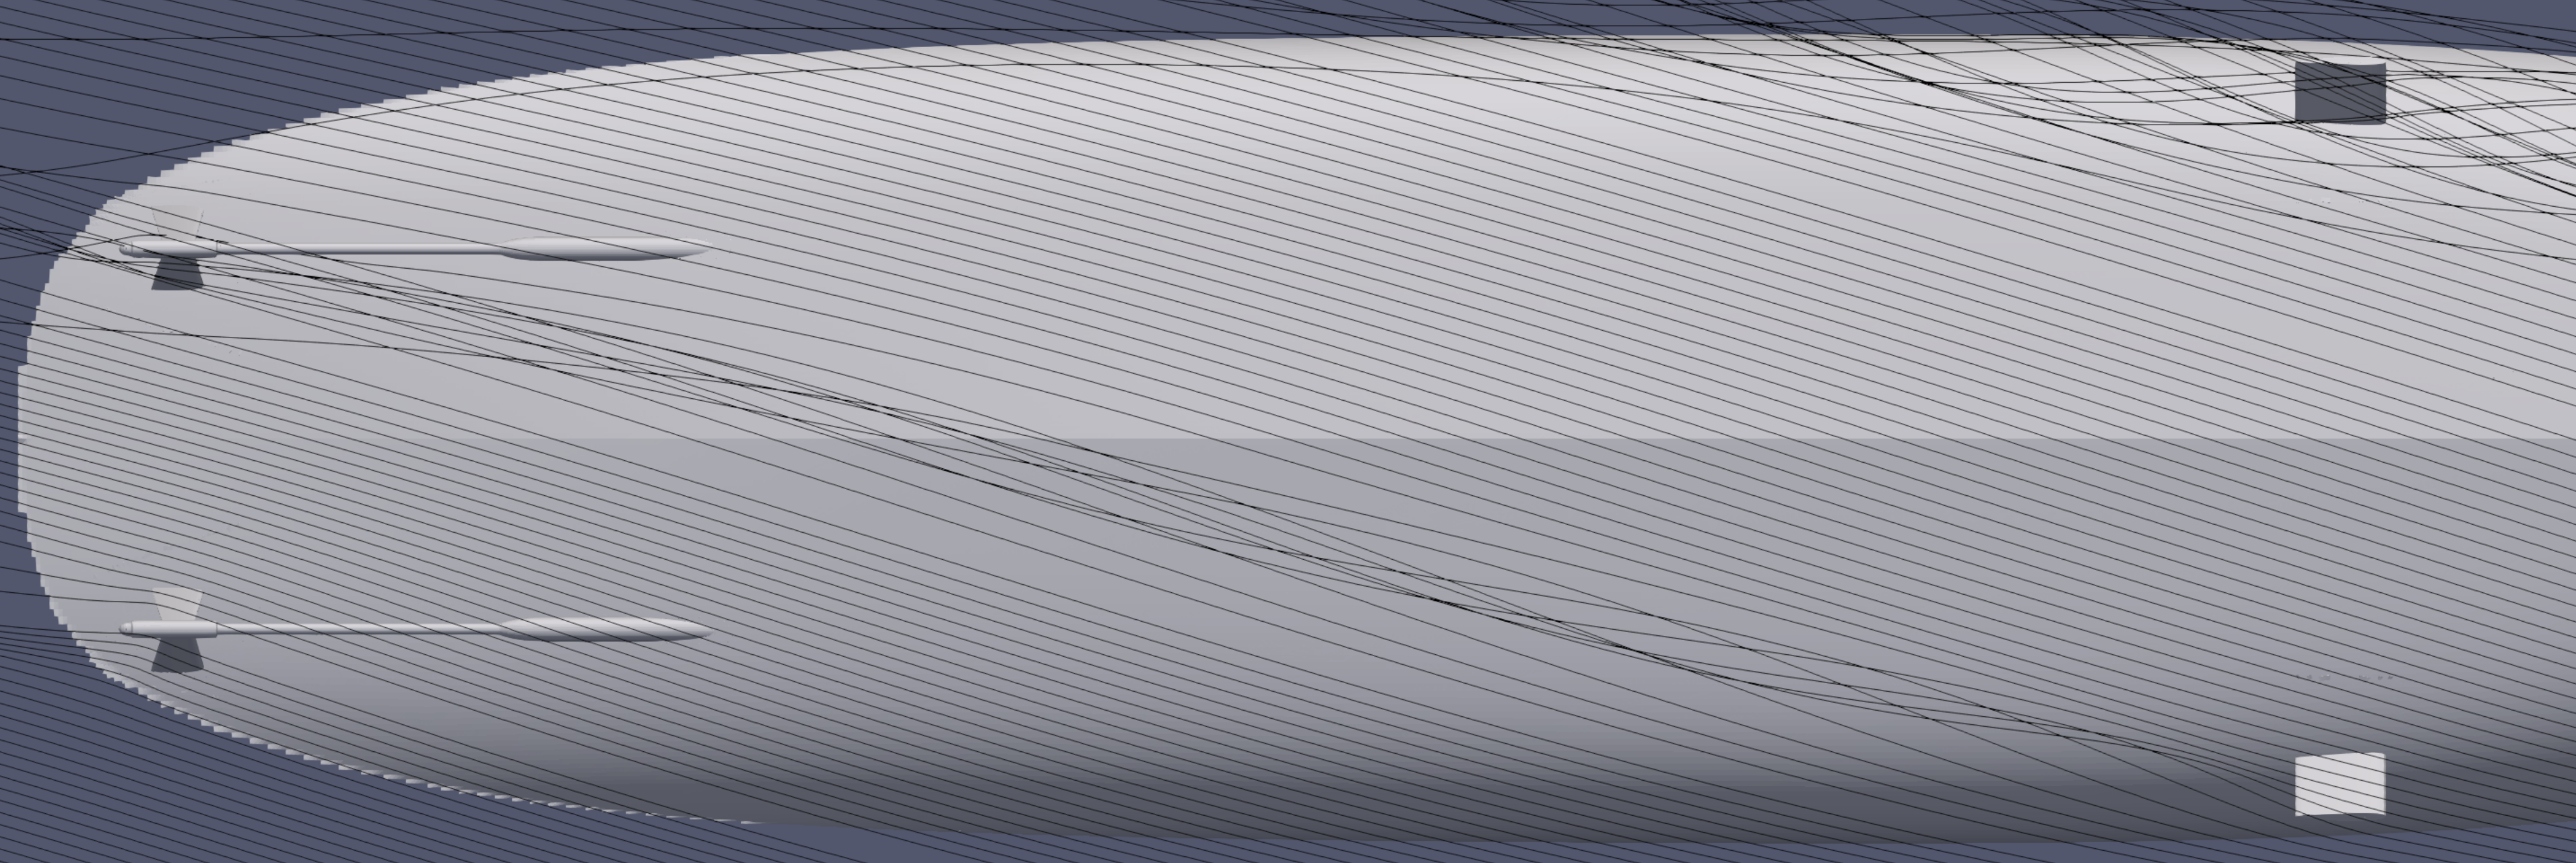
\includegraphics[width=\textwidth]{figures/paraview_drift_15.png}
    \caption{Streamlines for wPCC at 15 degrees drift angle.}
    \label{fig:streamlines15}
\end{figure}
%\FloatBarrier

\subsection{Inverse dynamics analysis wPCC}
Forces predicted with the wPCC model equipped with either the semi-empirical rudder or the polynomial rudder have been compared with forces from the experiment, estimated by inverse dynamics. Both rudder models have reasonably good agreement with the experimental results from the zigzag10/10 test (see \autoref{fig:ID_wPCC_10}). For the 20/20 test, only the polynomial rudder model seems to capture the forces correctly (see \autoref{fig:ID_wPCC_20}). There are however some yawing moment $N_D$ deviations during the rudder transitions at t=9.5 s, and t=27 s.

\begin{figure}
     \centering
     \begin{subfigure}[b]{\textwidth}
         \centering
         \includesvg{figures/results_wPCC_ID.zigzag 10_10.svg}
        \caption{Zigzag10/10 to port.}
        \label{fig:ID_wPCC_10}
     \end{subfigure}
     \vfill
     \begin{subfigure}[b]{\textwidth}
         \includesvg{figures/results_wPCC_ID.zigzag 20_20.svg}
        \caption{Zigzag20/20 to starboard.}
        \label{fig:ID_wPCC_20}
     \end{subfigure}
        \caption{Comparison between forces during zigzag tests estimated with inverse dynamics from the experiments and predictions with a model equipped with either a polynomial rudder or semi-empirical rudder model. Forces from VCT calculations of some interesting states have also been added.}
        \label{fig:ID_wPCC}
\end{figure}
\FloatBarrier
\subsection{Closed loop simulations wPCC}
\noindent As a complement to the inverse dynamics analysis, closed loop simulations were conducted for the wPCC. The simulation results are shown in \autoref{fig:sim_wPCC}. The results look quite similar to the inverse dynamic analysis presented above. The zigzag periods of the semi-empirical model were too short compared to the experiments and the overshoot angles were over-predicted up to three degrees. For the 10/10 zigzag test, by using the semi-empirical rudder to perform the close-loop maneuvering simulations, the over-prediction for both the first and second overshoot angles is about 1 degree. While for the 20/20 zigzag test, there is an increasing trend of over-prediction angles, i.e., less than 2 degrees over-prediction for the first overshoot angle, but up to 3 degrees discrepancy for the second overshoot angle. As explained before, this might be caused by the semi-empirical models to estimate rudder forces, as well as the asymmetric flow applied on the two rudders during the drifting operations.
\begin{figure}[h]
     \centering
     \begin{subfigure}[b]{\textwidth}
         \centering
         \includesvg[height=0.3\textheight]{figures/results_wPCC_ID.closed loop zigzag 10_10 port.svg}
        \caption{Simulations wPCC Zigzag10/10 to port.}
        \label{fig:sim_wPCC_10}
     \end{subfigure}
     \vfill
     \begin{subfigure}[b]{\textwidth}
        \centering
        \includesvg[height=0.3\textheight]{figures/results_wPCC_ID.closed loop zigzag 20_20 stbd.svg}
        \caption{Simulations wPCC Zigzag20/20 to starboard.}
        \label{fig:sim_wPCC_20}
     \end{subfigure}
        \caption{Comparison between zigzag tests with wPCC from experiments and simulations with a model equipped with either a polynomial rudder or semi-empirical rudder model.}
        \label{fig:sim_wPCC}
\end{figure}
%\begin{figure}[h]
%     \centering
%     \begin{subfigure}[b]{\textwidth}
%         \centering
%         \includesvg{figures/results_wPCC_ID.overshoot1.svg}
%        \caption{First overshoot angles.}
%        \label{fig:overhoots1_wPCC}
%     \end{subfigure}
%     \vfill
%     \begin{subfigure}[b]{\textwidth}
%         \centering
%         \includesvg{figures/results_wPCC_ID.overshoot2.svg}
%        \caption{Second overshoot angles.}
%        \label{fig:overhoots2_wPCC}
%     \end{subfigure}
%     
%        \caption{Overshoot angles from the wPCC experiments and simulations.}
%        \label{fig:overshoots_wPCC}
%\end{figure}
\FloatBarrier

\subsection{VCT Optiwise}
\noindent A series of fast VCTs with test scenarios as listed in \autoref{tab:VCT_optiwise} were conducted with CFD in Shipflow. Rudder force predictions with the MMG original rudder model and the modified MMG quadratic model were compared to VCT data for the rudder angle variation as shown in \autoref{fig:rudder_angle_compare_optiwise}. The newly added initial inflow angle parameter $\gamma_0$ (see \autoref{eq:gamma_R2}) allows the MMG quadratic model to be better adapted to the VCT data. However, the difference between the models is less obvious when looking at the thrust variation tests in \autoref{fig:rudder_angle_compare_optiwise_all}.
%gamma_0, thrust_variation
\begin{figure}[h]
     \centering
     \begin{subfigure}[b]{0.49\textwidth}
         \centering
         \includesvg{figures/results_optiwise_VCT.rudder_angle.svg}
        \caption{Rudder angle variation.}
        \label{fig:rudder_angle_compare_optiwise}
     \end{subfigure}
     \hfill
     \begin{subfigure}[b]{0.49\textwidth}
         \centering
         \includesvg{figures/results_optiwise_VCT.thrust_variation.svg}
        \caption{Thrust variation at \textpm 10 degrees rudder angle.}
        \label{fig:thrust_variation_optiwise}
     \end{subfigure}
    \caption{Rudder angle variation and thrust variation.}
    \label{fig:rudder_angle_compare_optiwise_all}
\end{figure}
\FloatBarrier

The results of the drift, circle tests and the circle and drift tests are used to validate the MMG model improved by this study (named the MMG quadratic) for the prediction of the rudder forces.
The newly added quadratic relationship for the flow straightening coefficient $\gamma_R$ (\autoref{eq:gamma_R2}) in the MMG quadratic rudder model fits better to the VCT data than the original MMG rudder model, as shown in \autoref{fig:MMG_quadratic}.
%beta_R
\begin{figure}[h]
     \centering
     \begin{subfigure}[b]{0.49\textwidth}
         \centering
         \includesvg{figures/results_optiwise_VCT.Y_R_MMG_original.svg}
        \caption{Original MMG rudder model.}
        \label{fig:Y_R_MMG_original}
     \end{subfigure}
     \hfill
     \begin{subfigure}[b]{0.49\textwidth}
         \centering
         \includesvg{figures/results_optiwise_VCT.Y_R_MMG_quadratic.svg}
        \caption{Modified quadratic MMG rudder model.}
        \label{fig:Y_R_MMG_quadratic}
     \end{subfigure}
    \caption{Rudder force during the VCT tests as a function of the effective inflow angle for the original MMG model and the modified quadratic MMG model.}
    \label{fig:MMG_quadratic}
\end{figure}

The side force generated both on the rudder and the hull surface during various VCT analyses as listed in Table \ref{tab:VCT_optiwise} were used to validate the identified manoeuvring model by the proposed procedure for the Optiwise as in \autoref{fig:VCT_optiwise}. The results of the side forces for various rudder angle tests are presented in \autoref{fig:rudder_angle_X_optiwise} -- \autoref{fig:rudder_angle_N_optiwise}, where all the forces are well predicted by the model through the rudder hull interaction coefficients $x_R$ and $a_R$. 
The model predicts zero rudder drag when the rudder angle is zero at straight ahead condition as shown in \autoref{fig:rudder_angle_X_optiwise}. This is because the MMG rudder model has no base drag coefficient like the semi-empirical rudder model for the wPCC (see \autoref{fig:drift_angle_X_wPCC}).
Similar comparisons are shown for the drift angle tests in \autoref{fig:drift_angle_X_optiwise} -- \autoref{fig:drift_angle_N_optiwise} and the circle tests in \autoref{fig:circle_X_optiwise} -- \autoref{fig:circle_N_optiwise}. 
\begin{figure}[h]
    \centering
    %Rudder angle
    \begin{subfigure}[b]{0.325\textwidth}
         \centering
         \includesvg[width=1.2 in]{figures/results_optiwise_VCT.rudder_angle_X.svg}
        \caption{X for Rudder angle tests}
        \label{fig:rudder_angle_X_optiwise}
    \end{subfigure}
    \hfill
    \begin{subfigure}[b]{0.325\textwidth}
        \centering
        \includesvg{figures/results_optiwise_VCT.rudder_angle_Y.svg}
       \caption{Y for Rudder angle tests}
       \label{fig:rudder_angle_Y_optiwise}
    \end{subfigure}
    \hfill
    \begin{subfigure}[b]{0.325\textwidth}
        \centering
        \includesvg{figures/results_optiwise_VCT.rudder_angle_N.svg}
       \caption{N for Rudder angle tests}
       \label{fig:rudder_angle_N_optiwise}
    \end{subfigure}

    \vfill
    %Drift angle
    \begin{subfigure}[b]{0.325\textwidth}
        \centering
        \includesvg{figures/results_optiwise_VCT.drift_angle_X.svg}
       \caption{X for Drift angle tests}
       \label{fig:drift_angle_X_optiwise}
    \end{subfigure}
    \hfill
    \begin{subfigure}[b]{0.325\textwidth}
        \centering
        \includesvg{figures/results_optiwise_VCT.drift_angle_Y.svg}
       \caption{Y for Drift angle tests}
       \label{fig:drift_angle_Y_optiwise}
    \end{subfigure}
    \hfill
    \begin{subfigure}[b]{0.325\textwidth}
        \centering
        \includesvg{figures/results_optiwise_VCT.drift_angle_N.svg}
       \caption{N for Drift angle tests}
       \label{fig:drift_angle_N_optiwise}
    \end{subfigure}
    
    \vfill
    %Circle
    \begin{subfigure}[b]{0.325\textwidth}
        \centering
        \includesvg{figures/results_optiwise_VCT.circle_X.svg}
       \caption{X for Circle tests}
       \label{fig:circle_X_optiwise}
    \end{subfigure}
    \hfill
    \begin{subfigure}[b]{0.325\textwidth}
        \centering
        \includesvg{figures/results_optiwise_VCT.circle_Y.svg}
       \caption{Y for Circle tests}
       \label{fig:circle_Y_optiwise}
    \end{subfigure}
    \hfill
    \begin{subfigure}[b]{0.325\textwidth}
        \centering
        \includesvg{figures/results_optiwise_VCT.circle_N.svg}
       \caption{N for Circle tests}
       \label{fig:circle_N_optiwise}
    \end{subfigure}
    
    \caption{Forces on the Optiwise analyzed by VCT (dots) and predictions from the identified model (lines).}
    \label{fig:VCT_optiwise}
\end{figure}
\FloatBarrier

\vspace{-0.5cm}
It should also be noted that the coupling terms $Y_{vrr}$,$Y_{vvr}$,$N_{vrr}$, and $N_{vvr}$ play an important role in accurately modeling the forces. As shown in \autoref{fig:circle_drift_optiwise}, by considering those coupling terms, the sway forces and yaw moments obtained from the identified model give better results than no-coupling models for those circle and drift captive tests.
\begin{figure}[ht]
    \centering
    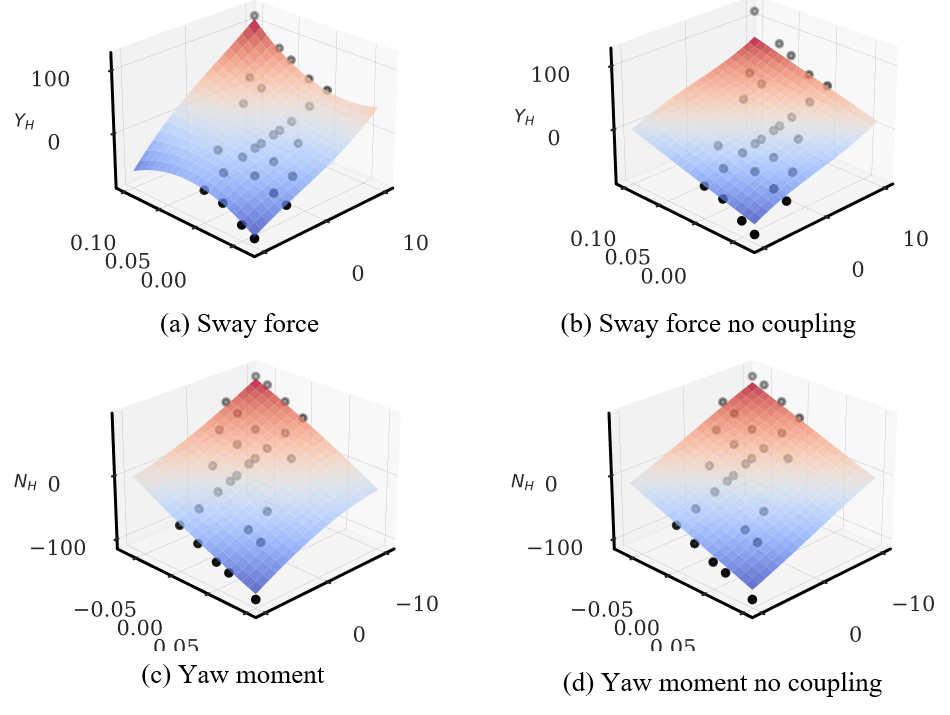
\includegraphics[width=0.7\linewidth]{figures/results_optiwise_vct.YNH.png}
    \caption{Optiwise hull forces during the circle and drift variations with/without the coupling terms, VCT (dots), fitted model (surface).}
    \label{fig:circle_drift_optiwise}
\end{figure}
\FloatBarrier

% % Circle + drift
% \begin{figure}[h]
%      \centering
%      \begin{subfigure}[b]{0.49\textwidth}
%          \centering
%          \includesvg{figures/results_optiwise_VCT.Y_H.svg}
%         \caption{Sway force.}
%         \label{fig:circle_drift_Y_H_optiwise}
%      \end{subfigure}
%      \hfill
%      \begin{subfigure}[b]{0.49\textwidth}
%          \centering         \includesvg{figures/results_optiwise_VCT.Y_H_no_coupling.svg}
%         \caption{Sway force no coupling.}
%         \label{fig:circle_drift_Y_H_no_coupling_optiwise}
%      \end{subfigure}
     
%      \vfill
%      \begin{subfigure}[b]{0.49\textwidth}
%          \centering
%          \includesvg{figures/results_optiwise_VCT.N_H.svg}
%         \caption{Yawing moment.}
%         \label{fig:circle_drift_N_H_optiwise}
%      \end{subfigure}
%      \hfill
%      \begin{subfigure}[b]{0.49\textwidth}
%          \centering
%          \includesvg{figures/results_optiwise_VCT.N_H_no_coupling.svg}
%         \caption{Yawing moment no coupling.}
%         \label{fig:circle_drift_N_H_no_coupling_optiwise}
%      \end{subfigure}
     
%     \caption{Optiwise hull forces during the circle and drift variations with/without the coupling terms, VCT (dots), fitted model (surface).}
%     \label{fig:circle_drift_optiwise}
% \end{figure}
\FloatBarrier

\subsection{Inverse dynamics analysis Optiwise}
FRMT experiments with Optiwise were conducted as a continuation of the wPCC experiments. During these tests, rudder forces were measured during the experiments, to get a better understanding of the rudder forces during the maneuvers. Prediction models equipped with the semi-empirical rudder, the MMG rudder, or the polynomial rudder were developed. A fourth model was also developed, which uses the actual measured rudder force instead of a prediction model -- so that only the hull forces need to be predicted. 

%10/10
The total forces acting on the ship during the FRMT experiments were estimated with inverse dynamics, in the same way as how the wPCC results were analyzed. There was generally good agreement for the zigzag10/10, as shown in \autoref{fig:ID_optiwise10}. Deviations were however observed for the sway force $Y_D$ during about 3 seconds after the rudder changes at t=11--14 s, and t=35--38 s, as indicated in \autoref{fig:ID_optiwise10}. All of the models and the VCT calculations predict a more straight line in the $Y_D$ time series around these deviation points. 
A reasonable explanation to these deviations has not been found during the work for this paper, where filtration errors in the EKF were ruled out as a possible explanation, by conducting alternative analysis with a low-pass filter instead of the EKF. Accelerations were instead calculated with numeric differentiation of the low-pass filtered signals of repeated zigzag10/10 tests as shown in \autoref{fig:lowpass_deviation_points}.
\begin{figure}[h]
    \centering
    \begin{subfigure}[b]{\textwidth}
        \centering
        \includesvg{figures/results_optiwise_ID.measured_rudder_zigzag 10_10.svg}
        \caption{Zigzag10/10 to port.}
        \label{fig:ID_measured_rudder_zigzag_10_10}
    \end{subfigure}
     \vfill
    \begin{subfigure}[b]{\textwidth}
        \centering
        \includesvg{figures/results_optiwise_ID.measured_rudder_zigzag 20_20.svg}
        \caption{Zigzag20/20 to starboard.}
        \label{fig:ID_measured_rudder_zigzag_20_20}
    \end{subfigure}
    \caption{Inverse dynamics forces during the zigzag tests compared to predictions with the measured rudder model.}
    \label{fig:ID_optiwise20}
\end{figure}
%20/20
The force predictions for the zigzag20/20 is shown in \autoref{fig:ID_optiwise20}. Similar deviations as for the zigzag10/10 were observed for $Y_D$ after the rudder changes (t=11--14 s, t=35--38 s, t=64 s). The yawing moment $N_D$ was not well predicted for the MMG rudder in the end of the port turn (t=23--33 s), where the other models had better agreement with the experiments. When the ship started to turn back to starboard (t=43--62 s) only the measured rudder forces model and the polynomial rudder agreed well with the experiments. Just as for wPCC, the total yawing moment $N_D$ deviations seem to originate from the rudder yawing moment $N_R$ predictions.
\begin{figure}[h]
    \centering
    \includesvg{figures/results_optiwise_deviation_points.lowpass.svg}
    \caption{Inverse dynamics sway force from repeated zigzag10/10 test to port. The accelerations have been estimated with the EKF and also with numeric differentiation of low-pass filtered signals.}
    \label{fig:lowpass_deviation_points}
\end{figure}



%\begin{figure}[h]
%     \centering
%     \begin{subfigure}[b]{\textwidth}
%         \centering
%         \includesvg{figures/results_optiwise_ID.zigzag 10_10.svg}
%        \caption{Forces Optiwise Zigzag10/10 to port.}
%        \label{fig:ID_optiwise10}
%     \end{subfigure}
%     \vfill
%     \begin{subfigure}[b]{\textwidth}
%         \includesvg{figures/results_optiwise_ID.zigzag 20_20.svg}
%        \caption{Forces Optiwise Zigzag20/20 to starboard.}
%        \label{fig:ID_optiwise20}
%     \end{subfigure}
%        \caption{Comparison between forces during zigzag tests with Optiwise estimated with inverse dynamics from the experiments and predictions with a model equipped with either a polynomial rudder or semi-empirical rudder model. Forces from VCT calculations of some interesting states have also been added.}
%        \label{fig:ID_optiwise}
%\end{figure}


\FloatBarrier
\subsection{Closed loop simulations Optiwise}
The results of closed-loop simulations with the Optiwise simulation model equipped with either the MMG original or the quadratic model are shown in \autoref{fig:sim_optiwise}. There was very good agreement for the zigzag20/20 tests and a little less agreement for the zigzag10/10 tests, where the MMG quadratic was the better of the two models. Up to four degrees of deviation was observed between the overshoot angles, as shown in \autoref{fig:overshoots_optiwise}.   
\begin{figure}[h]
     \centering
     \begin{subfigure}[b]{0.40\textwidth}
         \centering
         \includesvg{figures/results_optiwise_ID.closed loop zigzag 10_10 port.svg}
        \caption{Zigzag10/10 to port.}
        \label{fig:sim_optiwise_10_port}
     \end{subfigure}
     \hfill
     \begin{subfigure}[b]{0.40\textwidth}
         \includesvg{figures/results_optiwise_ID.closed loop zigzag 10_10 stbd.svg}
        \caption{Zigzag10/10 to starboard.}
        \label{fig:sim_optiwise_10_stbd}
     \end{subfigure}
     \vfill
     \begin{subfigure}[b]{0.40\textwidth}
         \centering
         \includesvg{figures/results_optiwise_ID.closed loop zigzag 20_20 port.svg}
        \caption{Zigzag20/20 to port.}
        \label{fig:sim_optiwise_20_port}
     \end{subfigure}
     \hfill
     \begin{subfigure}[b]{0.40\textwidth}
         \includesvg{figures/results_optiwise_ID.closed loop zigzag 20_20 stbd.svg}
        \caption{Zigzag20/20 to starboard.}
        \label{fig:sim_optiwise_20_stbd}
     \end{subfigure}
     
        \caption{Comparison of zigzag tests between experiments and simulations with the MMG rudder models.}
        \label{fig:sim_optiwise}
\end{figure}
\vspace{-1cm}

\begin{figure}[b!]
    \centering
    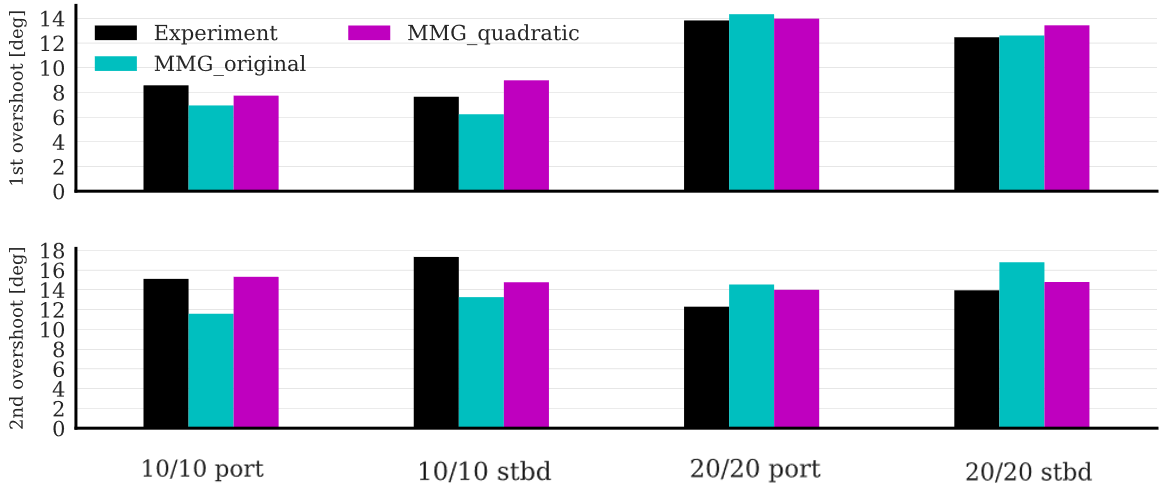
\includegraphics[width=0.9\linewidth, height = 5cm]{figures/results_optiwise_overshoot.png}
    \caption{Overshoot angles from the Optiwise experiments and simulations.}
    \label{fig:overshoots_optiwise}
\end{figure}
\vspace{-0.5cm}
% \begin{figure}[h]
%      \centering
%      \begin{subfigure}[b]{\textwidth}
%          \centering
%          \includesvg{figures/results_optiwise_ID.overshoot1.svg}
%         \caption{First overshoot angles.}
%         \label{fig:overhoots1_optiwise}
%      \end{subfigure}
%      \vfill
%      \begin{subfigure}[b]{\textwidth}
%          \centering
%          \includesvg{figures/results_optiwise_ID.overshoot2.svg}
%         \caption{Second overshoot angles.}
%         \label{fig:overhoots2_optiwise}
%      \end{subfigure}
     
%         \caption{Overshoot angles from the Optiwise experiments and simulations.}
%         \label{fig:overshoots_optiwise}
% \end{figure}
\FloatBarrier

\subsection{Rudder inflow analysis Optiwise}
The rudder inflow angle $\gamma$ and velocity $V_R$ were investigated by conducting a set of separate VCT calculations where the rudder was removed, so that an undisturbed flow by the rudder could be observed. The longitudinal and transverse inflow velocities $u_R$ and $v_R$ were measured along the rudder stock from the root to the tip of the rudder. \autoref{fig:rudder_velocities_span} shows the inflow velocity $\gamma=atan(v_R/u_R)$ along the rudder stock during four of the VCTs. The inflow angle varies a lot along the rudder span, from -27 to +27 degrees, around much smaller average angles of about \textpm 2.5-3 degrees. A positive inflow angle is generated above the clockwise rotating propeller and a negative angle is generated below it.
Rudder forces have been calculated with the MMG rudder model, where the expressions to calculate $u_R$ and $v_R$ have been replaced by measured values. 
\begin{figure}[h]
    \centering 
    \includesvg{figures/results_optiwise_rudder_velocities.inflow_angle.svg}
    \caption{Rudder inflow angle from the root to the tip of the rudder during two circle tests.}
     \label{fig:rudder_velocities_span}
\end{figure}
\begin{figure}[h]
     \centering
     \begin{subfigure}[b]{\textwidth}
         \centering
         \includesvg{figures/results_optiwise_rudder_velocities.drift_angle.svg}
        \caption{Drift angle.}
        \label{fig:inflow_to_force_drift_angle}
     \end{subfigure}
     \vfill
     \begin{subfigure}[b]{\textwidth}
         \includesvg{figures/results_optiwise_rudder_velocities.circle.svg}
        \caption{Circles.}
        \label{fig:inflow_to_force_circle}
     \end{subfigure}
        \caption{Rudder forces from VCT and predictions from the measured inflow velocities.}
        \label{fig:inflow_to_rudder_force}
\end{figure}

\FloatBarrier


\section{Discussion}
\label{sec:discussion}


\section{Conclusions}
\label{sec:conclusions}
%_________________________________________________________
%Move 1: Background information (research purposes, theory,
%methodology)
%
\noindent Maneuvering models were developed for two WAPS test cases with large rudders. The models were identified by conducting VCTs to obtain the hydrodynamic damping coefficients and by conducting pure yaw and pure sway simulations in the FNPF to obtain the added masses. The identified force models were compared with the inverse dynamics forces of the zigzag tests to identify possible weak spots within the models.  

%%_________________________________________________________
%%Move 2: Summarizing and reporting key results. (oblig.)
The identified wPCC model was shown to be well adapted to the VCT data, where the importance of the coupling terms was also shown in the combined drift and yaw rate cases.
However, the FRMT inverse dynamics forces were quite different from the VCT data and the model predictions. From this it was concluded that there must be an inherent error in the VCT data for wPCC that was inherited by the identified hull force model.

The inherent error in the wPCC VCT data could originate from false assumptions about neglected wave generation and roll exclusion. Therefore, another test case, Optiwise, was investigated in which these assumptions were assumed to be more valid.

It was shown that a model, with the rudder model replaced by the actual measured rudder forces, predicted total forces that were similar to the total forces from the inverse dynamics. Hence, it was concluded that for Optiwise the hull force prediction was correct.

The newly proposed MMG quadratic rudder model was then shown to be identifiable from the VCT data to get good agreement, in fact even better than the original MMG rudder model, with the FRMT measured rudder forces and consequently also good agreement with the total forces. 
%_________________________________________________________
%Move 3: Commenting on key results (making claims, explaining the results,
%comparing the new work with previous studies, offering
%alternative explanations) (oblig.)
For Optiwise it can be concluded that the VCT data contained correct damping forces during the maneuvers, which were well described by the chosen model structure, and also that the method used to determine added masses gave reasonable values. 

This analysis of the wPCC and Optiwise test cases has shown that inverse dynamics together with state VCTs is an effective tool to identify and explain possible weak spots within the identified models.

%It was shown that the proposed way to determine added masses with FNPF pure yaw and pure sway tests
%
%added masses from the FNPF pure yaw and pure sway tests produced inverse dynamics forces that agreed well with the force prediction models and the state VCTs for the Optiwise test case, which suggests that this is an accurate way to determine the added masses.
%
%Two enhancements to the MMG rudder model were proposed which improved the fit to the VCT data and also gave a little bit better results in the closed loop simulations.
%The coupling terms between sway and yaw rate were important for both wPCC and Optiwise.

%_________________________________________________________
%Move 4: Stating the limitations of the study
It should also be mentioned that if completely new maneuvers are simulated, the models in this paper would need a propeller prediction model that would be self-containing.
%_________________________________________________________
%Move 5: Making recommendations for future implementation and/or for
%future research

\FloatBarrier

\section{Acknowledgements}
\noindent The authors would like to acknowledge Trafikverket (Swedish Transport Administration) and Lighthouse, swedish maritime competence centre (www.lighthouse.nu) for providing the resources to prepare this paper. They would also thank all personnel at SSPA Maritime Center who have been involved in creating the model test results, building the ship models, and conducting the experiments.

%% The Appendices part is started with the command \appendix;
%% appendix sections are then done as normal sections
\appendix


\FloatBarrier
%% If you have bibdatabase file and want bibtex to generate the
%% bibitems, please use
%%
\pagebreak
\bibliographystyle{elsarticle-harv}
%\bibliography{Paper_3_semiempirical_rudder.bib}
\bibliography{Paper_5.bib}

\end{document}

\endinput
%%
%% End of file `elsarticle-template-harv.tex'.
